\documentclass[tikz,border=12pt]{standalone}
\usepackage[T1]{fontenc}
\usepackage{mathpazo}
\usepackage{amsmath,amssymb}
\usetikzlibrary{arrows.meta, calc, patterns, decorations.pathreplacing}

\definecolor{stblue}{HTML}{7B97AD}
\definecolor{rwgold}{HTML}{B8995E}
\definecolor{sage}{HTML}{7A9A7E}
\definecolor{dkbrown}{HTML}{3D3530}
\definecolor{wmgray}{HTML}{7B7067}
\definecolor{cream}{HTML}{F9F6F0}
\definecolor{border}{HTML}{D4C9B8}
\definecolor{terracotta}{HTML}{C47A6A}
\definecolor{lavender}{HTML}{907EA0}
\definecolor{rosewood}{HTML}{AD8480}

\begin{document}
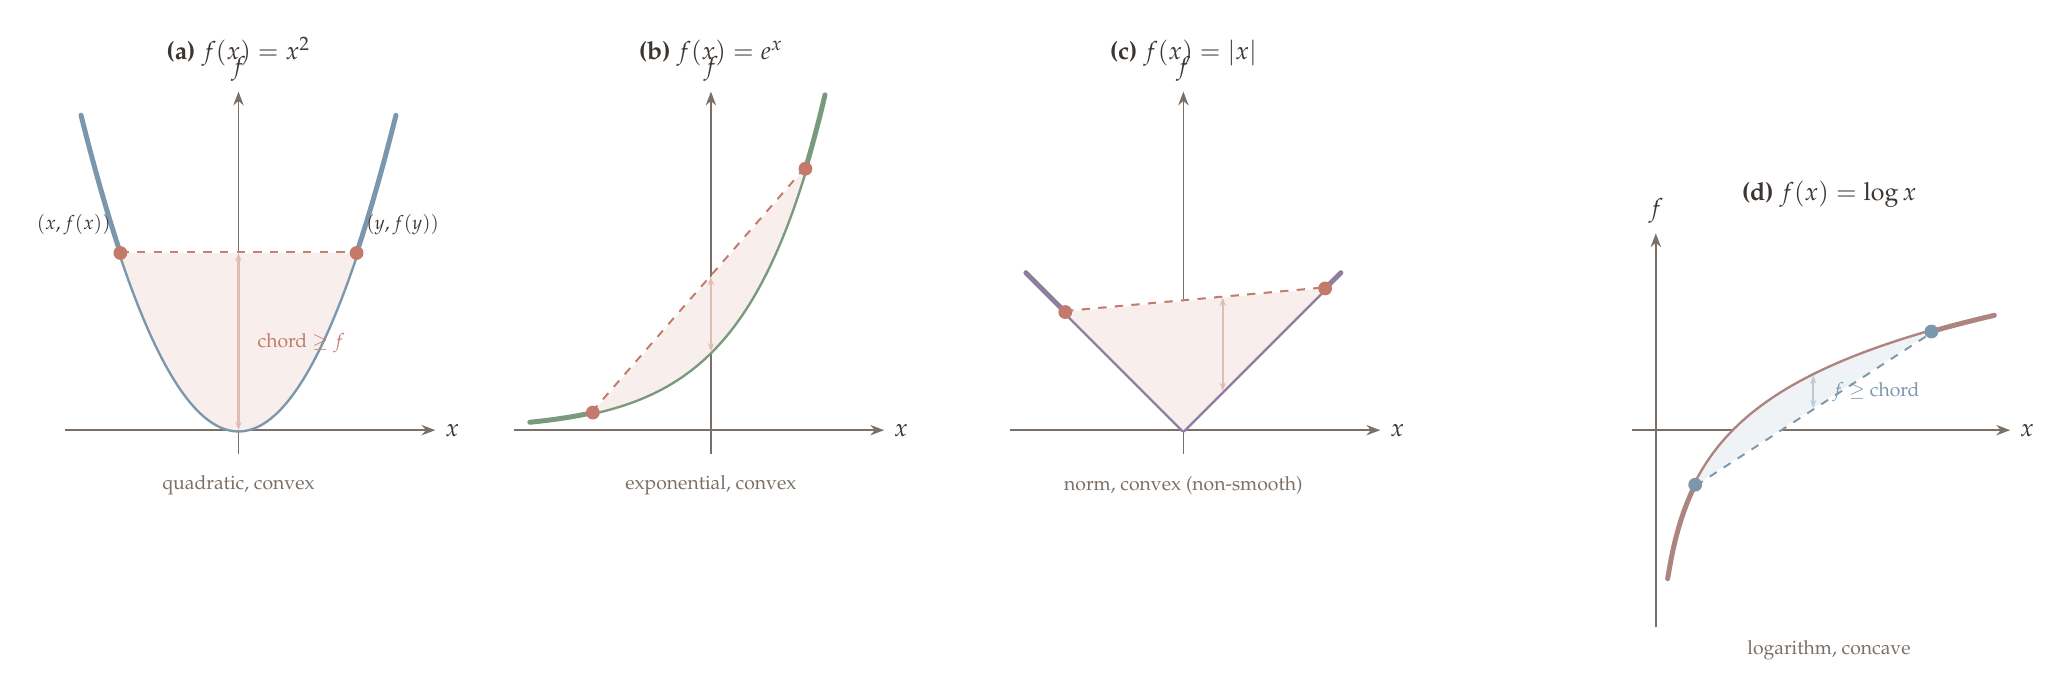
\begin{tikzpicture}[
  axis/.style={-{Stealth[length=5pt]}, wmgray, line width=0.6pt},
  curve/.style={line width=1.8pt, line cap=round},
  chord/.style={terracotta, line width=1.5pt, dashed},
  gap/.style={terracotta!50, line width=0.8pt, {Stealth[length=3pt]}-{Stealth[length=3pt]}},
  dot/.style={circle, fill=#1, inner sep=0pt, minimum size=5pt},
  label/.style={dkbrown, font=\small},
]

% ===== Panel (a): f(x) = x^2 with chord =====
\begin{scope}[shift={(0,0)}]
  \draw[axis] (-2.2,0) -- (2.5,0) node[right, label] {$x$};
  \draw[axis] (0,-0.3) -- (0,4.3) node[above, label] {$f$};

  % Curve
  \draw[curve, stblue, domain=-2:2, samples=80, smooth]
    plot (\x, {\x*\x});

  % Chord from (-1.5, 2.25) to (1.5, 2.25)
  \draw[chord] (-1.5, 2.25) -- (1.5, 2.25);

  % Shade region between chord and curve
  \fill[terracotta!12] (-1.5,2.25)
    -- plot[domain=-1.5:1.5, samples=60] (\x, {\x*\x})
    -- (1.5, 2.25) -- cycle;

  % Endpoints
  \node[dot=terracotta] at (-1.5, 2.25) {};
  \node[dot=terracotta] at (1.5, 2.25) {};

  % Labels on endpoints
  \node[dkbrown, font=\scriptsize, anchor=south east] at (-1.5, 2.35) {$(x, f(x))$};
  \node[dkbrown, font=\scriptsize, anchor=south west] at (1.5, 2.35) {$(y, f(y))$};

  % Gap arrow at midpoint
  \draw[gap] (0, 0) -- (0, 2.25);
  \node[terracotta, font=\scriptsize, anchor=west] at (0.12, 1.1) {chord $\geq f$};

  % Title
  \node[dkbrown, font=\small\bfseries, anchor=south] at (0, 4.5) {(a) $f(x) = x^2$};
  \node[wmgray, font=\scriptsize] at (0, -0.7) {quadratic, convex};
\end{scope}

% ===== Panel (b): f(x) = e^x with chord =====
\begin{scope}[shift={(6,0)}]
  \draw[axis] (-2.5,0) -- (2.2,0) node[right, label] {$x$};
  \draw[axis] (0,-0.3) -- (0,4.3) node[above, label] {$f$};

  % Curve: e^x scaled to fit
  \draw[curve, sage, domain=-2.3:1.45, samples=80, smooth]
    plot (\x, {exp(\x)});

  % Chord from (-1.5, e^{-1.5}) to (1.2, e^{1.2})
  \pgfmathsetmacro{\xa}{-1.5}
  \pgfmathsetmacro{\ya}{exp(-1.5)}
  \pgfmathsetmacro{\xb}{1.2}
  \pgfmathsetmacro{\yb}{exp(1.2)}
  \draw[chord] (\xa, \ya) -- (\xb, \yb);

  % Shade
  \fill[terracotta!12] (\xa,\ya)
    -- plot[domain=\xa:\xb, samples=60] (\x, {exp(\x)})
    -- (\xb, \yb) -- cycle;

  % Endpoints
  \node[dot=terracotta] at (\xa, \ya) {};
  \node[dot=terracotta] at (\xb, \yb) {};

  % Gap at x=0
  \pgfmathsetmacro{\chordatzero}{\ya + (0 - \xa)/(\xb - \xa)*(\yb - \ya)}
  \draw[gap] (0, 1) -- (0, \chordatzero);

  \node[dkbrown, font=\small\bfseries, anchor=south] at (0, 4.5) {(b) $f(x) = e^x$};
  \node[wmgray, font=\scriptsize] at (0, -0.7) {exponential, convex};
\end{scope}

% ===== Panel (c): f(x) = |x| with chord =====
\begin{scope}[shift={(12,0)}]
  \draw[axis] (-2.2,0) -- (2.5,0) node[right, label] {$x$};
  \draw[axis] (0,-0.3) -- (0,4.3) node[above, label] {$f$};

  % Curve: |x|
  \draw[curve, lavender, line join=round] (-2, 2) -- (0, 0) -- (2, 2);

  % Chord from (-1.5, 1.5) to (1.8, 1.8)
  \draw[chord] (-1.5, 1.5) -- (1.8, 1.8);

  % Shade
  \fill[terracotta!12] (-1.5, 1.5)
    -- (-1.5, 1.5) -- (0, 0) -- (1.8, 1.8) -- cycle;

  % Endpoints
  \node[dot=terracotta] at (-1.5, 1.5) {};
  \node[dot=terracotta] at (1.8, 1.8) {};

  % Gap
  \pgfmathsetmacro{\chordatpt}{1.5 + (0.5 - (-1.5))/(1.8 - (-1.5))*(1.8 - 1.5)}
  \draw[gap] (0.5, 0.5) -- (0.5, \chordatpt);

  \node[dkbrown, font=\small\bfseries, anchor=south] at (0, 4.5) {(c) $f(x) = |x|$};
  \node[wmgray, font=\scriptsize] at (0, -0.7) {norm, convex (non-smooth)};
\end{scope}

% ===== Panel (d): f(x) = log(x) CONCAVE =====
\begin{scope}[shift={(18,0)}]
  \draw[axis] (-0.3,0) -- (4.5,0) node[right, label] {$x$};
  \draw[axis] (0,-2.5) -- (0,2.5) node[above, label] {$f$};

  % Curve: ln(x) scaled
  \draw[curve, rosewood, domain=0.15:4.3, samples=80, smooth]
    plot (\x, {ln(\x)});

  % Chord from (0.5, ln(0.5)) to (3.5, ln(3.5))
  \pgfmathsetmacro{\xa}{0.5}
  \pgfmathsetmacro{\ya}{ln(0.5)}
  \pgfmathsetmacro{\xb}{3.5}
  \pgfmathsetmacro{\yb}{ln(3.5)}
  \draw[chord, stblue, dashed] (\xa, \ya) -- (\xb, \yb);

  % Shade -- chord BELOW curve for concave
  \fill[stblue!12] (\xa,\ya)
    -- plot[domain=\xa:\xb, samples=60] (\x, {ln(\x)})
    -- (\xb, \yb) -- cycle;

  % Endpoints
  \node[dot=stblue] at (\xa, \ya) {};
  \node[dot=stblue] at (\xb, \yb) {};

  % Gap at x=2
  \pgfmathsetmacro{\chordattwo}{\ya + (2 - \xa)/(\xb - \xa)*(\yb - \ya)}
  \draw[stblue!50, line width=0.8pt, {Stealth[length=3pt]}-{Stealth[length=3pt]}]
    (2, \chordattwo) -- (2, {ln(2)});
  \node[stblue, font=\scriptsize, anchor=west] at (2.12, {0.5*(\chordattwo + ln(2))}) {$f \geq$ chord};

  \node[dkbrown, font=\small\bfseries, anchor=south] at (2.2, 2.7) {(d) $f(x) = \log x$};
  \node[wmgray, font=\scriptsize] at (2.2, -2.8) {logarithm, concave};
\end{scope}

\end{tikzpicture}
\end{document}
